\documentclass[11pt, a4paper]{MATH2023}
\usepackage{fancyhdr}
\usepackage{setspace}
\usepackage{amsmath,mathrsfs}
\usepackage{multicol}
\usepackage{amssymb}
\usepackage{graphicx}
\usepackage{caption}
\usepackage{subcaption}
\usepackage{xcolor}
\usepackage{enumitem}
\usepackage{tikz}
\usepackage{mathtools}
\usetikzlibrary{matrix}
\usepackage[normalem]{ulem}
\usepackage{multirow}
\usepackage[linesnumbered, ruled, boxed]{algorithm2e}
\SetKwRepeat{Do}{do}{while}
\newcommand{\eg}{\textbf{[Example.] }}
\newcommand{\sol}{\textbf{[Solution.] }}
\newcommand{\vct}{\underline}
\newcommand{\vv}{\underline{v}}
\newcommand{\uu}{\underline{u}}
\newcommand{\ww}{\underline{w}}
\newcommand{\rr}{\underline{r}}
\newcommand{\ii}{\underline{i}}
\newcommand{\kk}{\underline{k}}
\newcommand{\jj}{\underline{j}}
\newcommand{\va}{\underline{a}}
\newcommand{\bb}{\underline{b}}
\newcommand{\cc}{\underline{c}}
\newcommand{\dd}{\underline{d}}

\title{Chapter 11}
\subtitle{Vector Functions and Curves}

\begin{document}
\begin{spacing}{1.3}

    \section{Vector Functions of One Variable}

    {\bf Vector-valued functions}: the value of the functions is a vector.
    Used to represent {\bf curves parametrically.}

    $$\rr=\rr(t)=x(t)\ii+y(t)\jj+z(t)\kk$$

    As $t$ varies, $\rr$ traces a {\bf space curve.} Such a curve is 
    called a {\bf parametric curve}.


    \section{Curves and Parametrizations}

    \eg The plane $x + y = 1$ intersects the paraboloid $z = x^2 + y^2$({\blue recall this is rice bowl})
    in a parabola. Parametrize the whole parabola using $t = x$ as parameter. 

    \sol Since $y=1-x$ and $z=x^2+y^2=1-2t+2t^2$, thus the required Parametrization is: 
    $$\rr(t)=t\ii+(1-t)\jj+(1-2t+2t^2)\kk,\ -\infty < t < \infty$$ 


    {\bf Parametrize the Curve of Intersection of Two Surfaces:}

    \eg Parametrize the curve of intersection of the plane $x +2y +4z = 4$ 
    and the elliptic cylinder $x^2 + 4y^2 = 4$.

    \sol We begin with the equation $x^2 +4y^2 = 4$, which is independent of $z$,
    $$x=2\cos t,\ y=\sin t,\ \ \red{(0\le t\le 2\pi)}$$
    then we can solve the equation for $z$: 
    $$z=\frac{1}{4}(4-x-2y)=1-\frac{1}{2}(\cos t+\sin t)$$
    thus the intersection of the given two surfaces is: 
    $$\rr (t)=2\cos t\ii + \sin t\jj+ \left(1-\frac{\cos t+\sin t}{2}\right)\kk,
    \ \ \red{(0\le t\le 2\pi)}$$

    \eg Find the parametric equations of the curve of intersection of the surfaces 
    $z=f(x,y)=a-x^2$ and $z=g(x,y)=a-y^2$.

    \sol Equal them to eliminate $a$, we get $y=\pm x$. Then let $x=t$, $y=\pm t$,
    $z=a-t^2$, so the equations will be: 
    $$\rr(t)=(t,t,a-t^2),\ \ {\rm or}\ \  \rr(t)=(t,-t,a-t^2)$$
    \begin{center}
        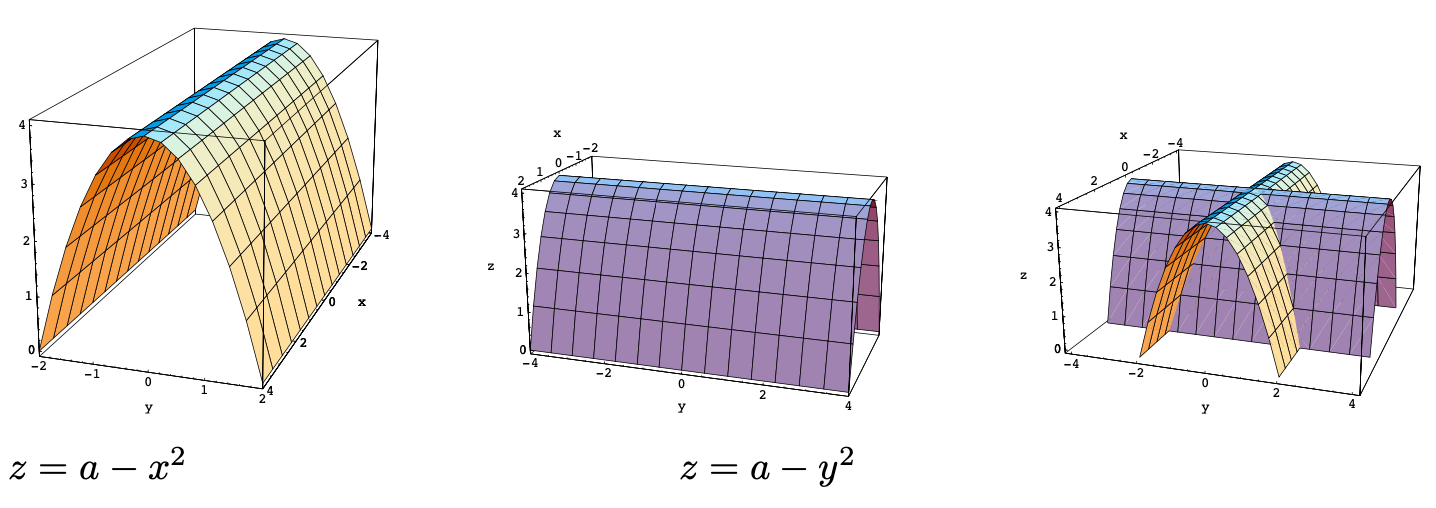
\includegraphics[scale=0.42]{images/Ch11-parametric-intersection-surfaces.png}
    \end{center}



    \section{Calculus of vector-valued functions}

    {\bf Limit:}
    $$\lim_{t\rar a}\rr(t)=\lim_{t\rar a}x(t)\ii+\lim_{t\rar a}y(t)\jj+\lim_{t\rar a}z(t)\kk$$

    {\bf Continuous:} at $a$ if $\disp \lim_{t\rar a}\rr(t)=\rr(a)$.

    {\bf Derivative: } 
    $$\rr'(t)=\lim_{h\rar 0}\frac{\rr(t+h)-\rr(t)}{h}=x'(t)\ii+y'(t)\jj+z'(t)\kk$$

    {\bf Rules of differentiation:}
    \begin{itemize}
        \item $(\vct{c})'=\vct{0}$
        \item addition and scalar multiplication: omit.
        \item $(f(t)\rr(t))'=f'(t)\rr(t)+f(t)\rr'(t)$
        \item $(\vct{r_1}(t)\cdot \vct{r_2}(t))'=\vct{r_1}'(t)\cdot \vct{r_2}(t)
        +\vct{r_1}(t)\cdot \vct{r_2}'(t)$
        \item $(\vct{r_1}(t)\times \vct{r_2}(t))'=\vct{r_1}'(t)\times \vct{r_2}(t)
        +\vct{r_1}(t)\times \vct{r_2}'(t)$
        \item {\bf chain rule:} $(\rr(f(t)))'=\rr'(f(t))\cdot f'(t)$
    \end{itemize}

    \eg Find $\disp \frac{d}{dt}||\rr(t)||.$

    \sol {\bf Method 1:}
    \begin{align*}
        \rr(t) &= (x(t), y(t), z(t))\\
        ||\rr(t)|| &= [x^2(t)+y^2(t)+z^2(t)]^{1/2}\\
        \frac{d}{dt}||\rr(t)|| &= \frac{1}{2}\cdot [x^2(t)+y^2(t)+z^2(t)]^{1/2}
        \cdot [2xx'+2yy'+2zz']\\
        &= \frac{1}{||\rr||}(x,y,z)\cdot (x',y',z')=\frac{\rr\cdot \rr'}{||\rr||}
    \end{align*}

    {\bf Method 2:} Notice $||\rr||^2=\rr\cdot \rr$,
    \begin{align*}
        \frac{d}{dt}||\rr||^2 &= \frac{d}{dt}(\rr\cdot \rr)\\
        2||\rr||\frac{d}{dt}||\rr|| &= \rr'\cdot \rr+\rr\cdot \rr'\\
        \frac{d}{dt}||\rr|| &= \frac{\rr\cdot \rr'}{||\rr||}
    \end{align*}

    \section{Higher order derivatives}
    \begin{itemize}
        \item Position: $\rr(t)$
        \item Velocity: $\disp \frac{d}{dt}\rr(t) = \rr'(t)$
        \item Acceleration: $\disp \frac{d}{dt}\rr'(t) = \rr''(t)$
    \end{itemize}


    \section{Arc Length}
    \begin{align*}
        ds &= \sqrt{\left(\frac{dx}{dt}\right)^2 + \left(\frac{dy}{dt}\right)^2} dt\\
        s &= \int_{t_1}^{t_2} \sqrt{\left(\frac{dx}{dt}\right)^2 + \left(\frac{dy}{dt}\right)^2} dt\\
        &= \int_{t_1}^{t_2} ||\rr'|| dt
    \end{align*}

    \eg find the position of a point on the parametric curve 
    $$\rr(t)=\cos^3t\ii+\sin^3t\jj+2\kk$$
    that has arc length $s$ unit from $\rr(0)=(1,0,2)$.

    \sol $$\int_{0}^{t_0}||\rr'(t)||dt=s,\ \ \rr'(t)=-3\cos^2t\sin t\ii+3\sin^2 t\cos t\jj$$
    $$s=\int_{0}^{t_0}(\cdots)dt=\frac{3}{2}\sin^2 t_0$$
    $$t_0=\sin^{-1}\sqrt{\frac{2s}{3}}$$
    

\end{spacing}
\end{document}
